\section{Conclusion of Problem Analysis}

During the research for this project, we have figured out what technologies we will use when solving our problem, that is stated in the W-diagram.
We will be using a rover to navigate around with multiple sensors. Making a 2D map of its surroundings, with the possibility of implementing equipment for 3D mapping. We will be using both sound and light sensors for navigation and mapping. Ultrasonic-sensors will be used for close encounter maneuvers for their high precision at a close range (up to 4m)\cite{ultra}. For mapping we will be using a laser sensor, that will either automatically turn 360$^{\circ}$  or we will implement a motor to rotate the sensor.
The rover will both be remote controlled and autonomous for navigation. For reference points we will be using the ultrasonic-sensors. The control computer will be a Raspberry Pi running a Debian Unix operating system. The reason for using the Raspberry Pi is that it can multi-task, read many sensors at the same time and build the 2D map on the go. For other microcontrollers, like the Arduino, we would only be able to collect data and need to build the map from it later, using another computer.

\begin{figure}[H]
	\centering
	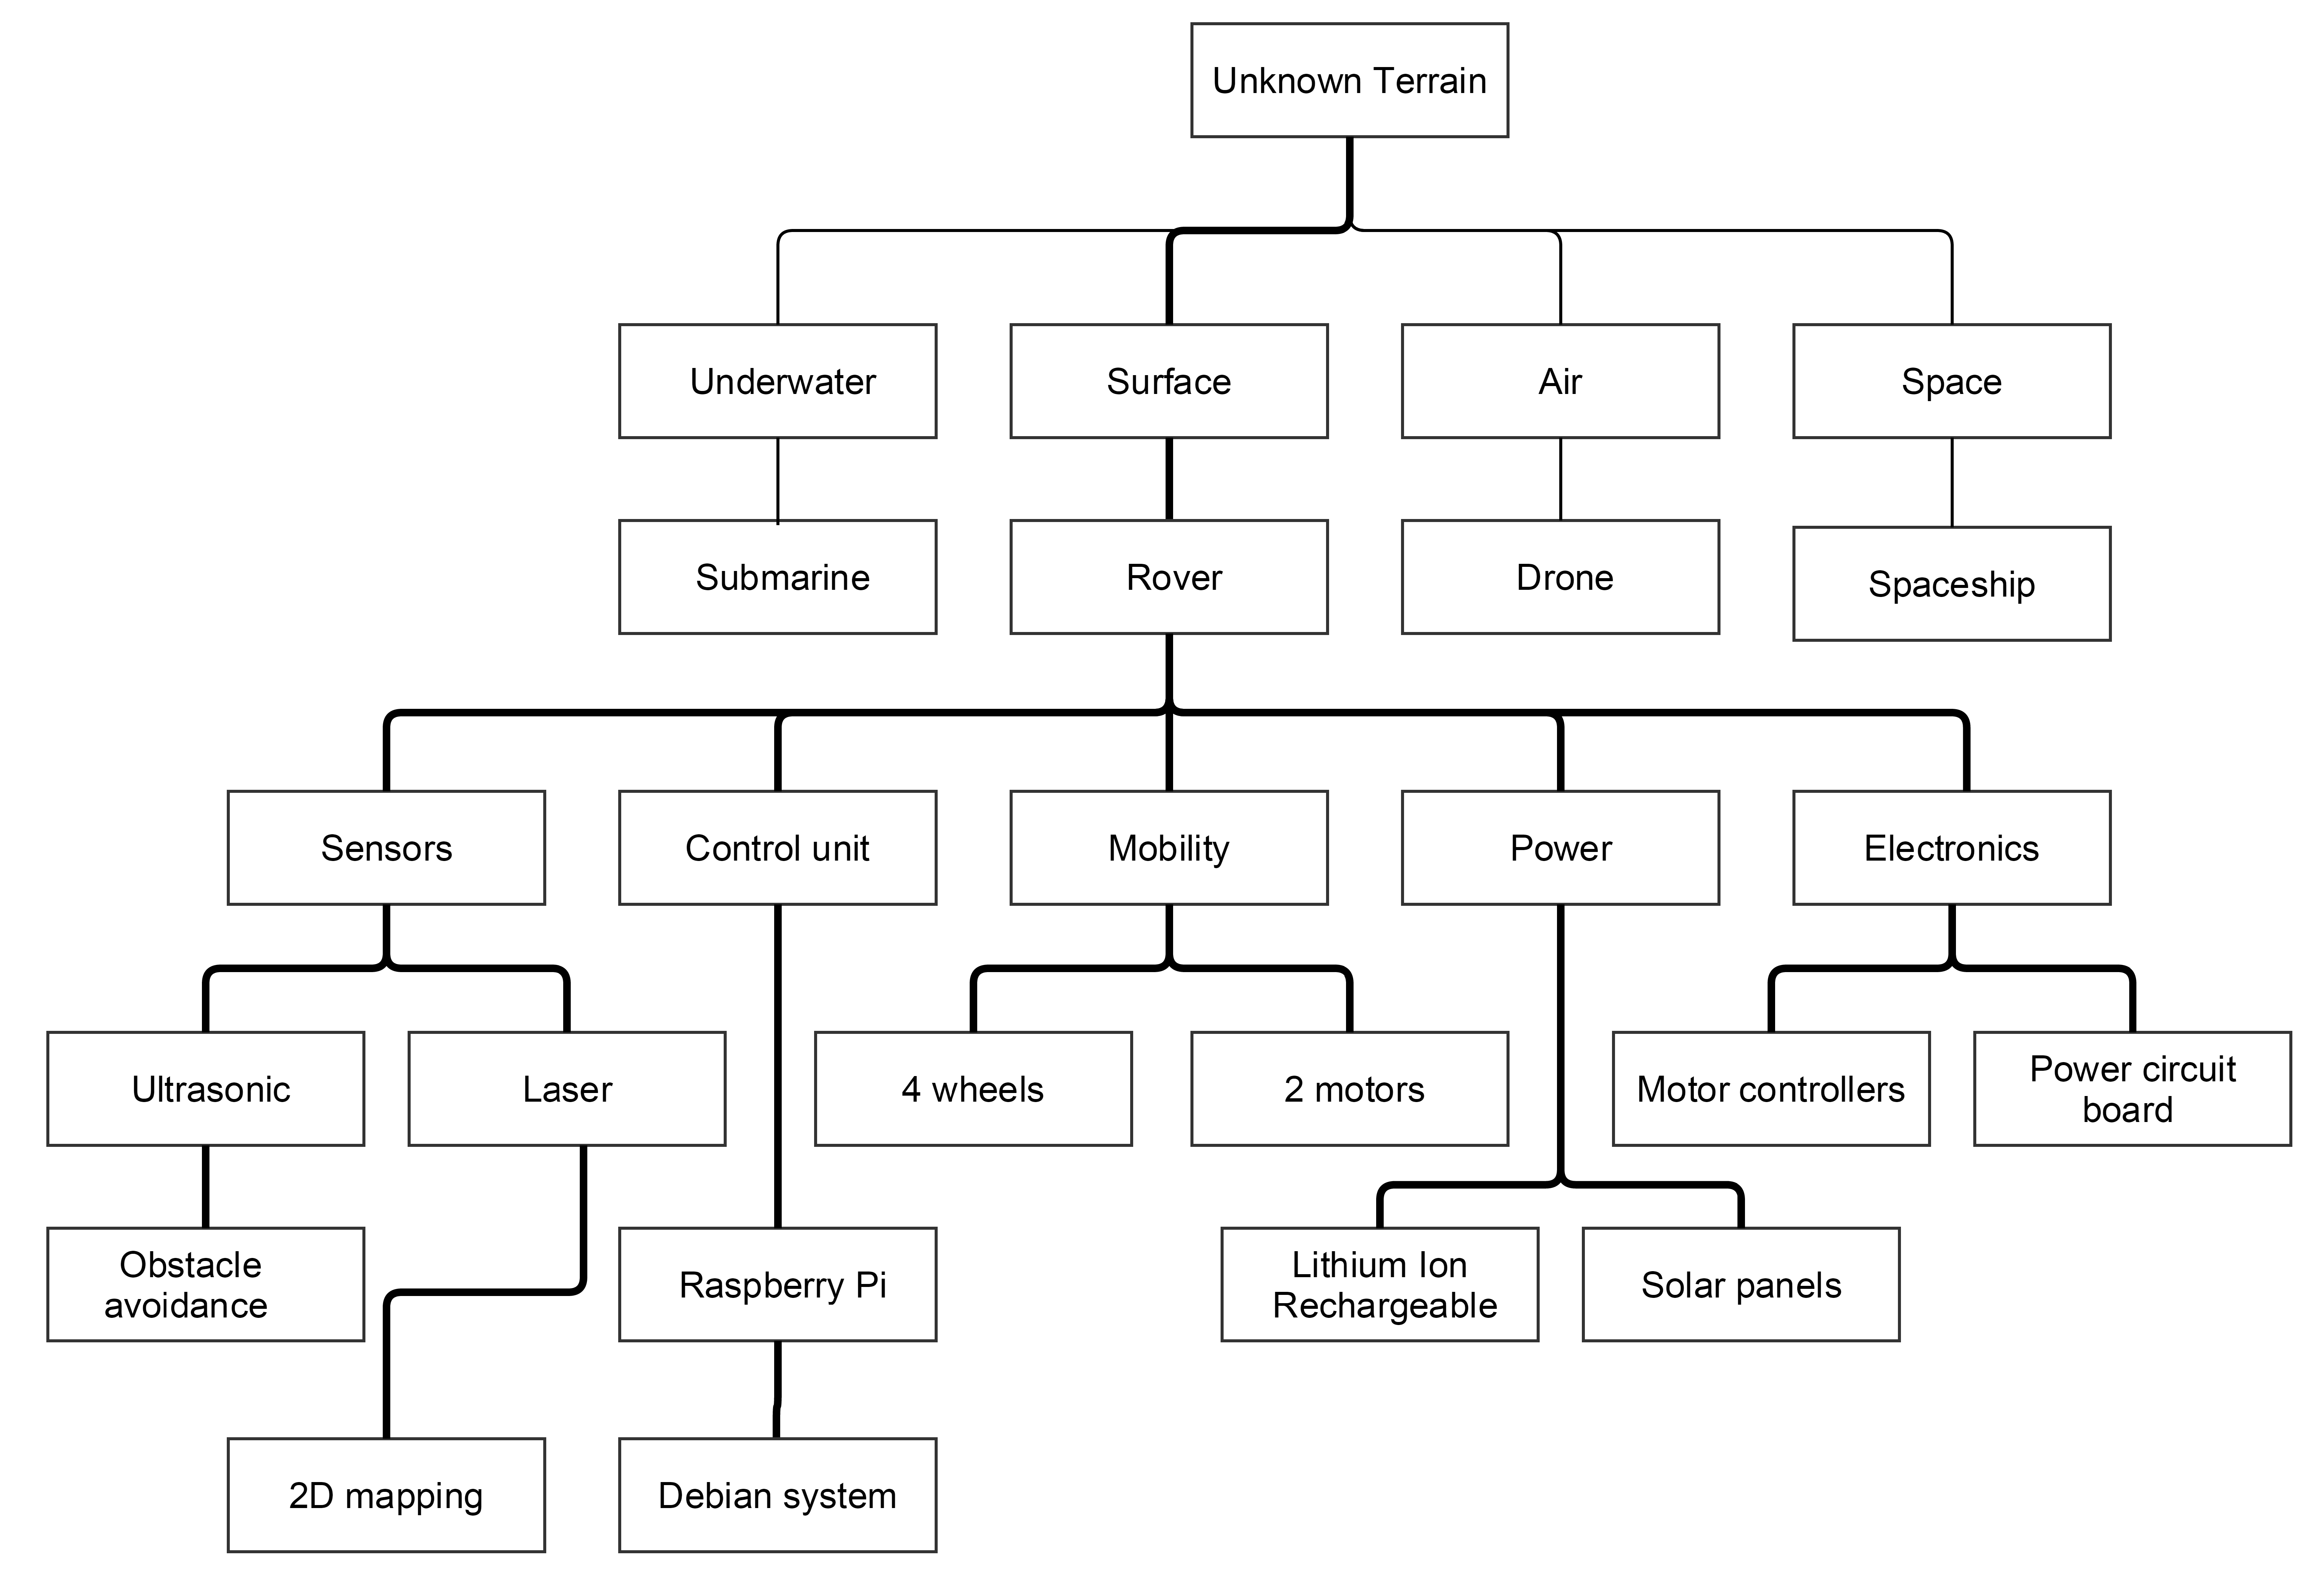
\includegraphics[scale=.1]{images/level3.png}
	\caption{Flowchart of the prototype idea.}
	\label{fig:level3}
\end{figure}

On this flowchart you can see how we expend from the flowchart we showed in chapter one. We decided to go the rover way and extended the requirements needed to full fill the requirements for a working prototype.

\clearpage
